\documentclass[12pt, titlepage]{article}
\usepackage{hyperref}
% Author's up-front packages
\usepackage[T1]{fontenc}
\usepackage[utf8]{inputenc}
\usepackage{longtable}
\usepackage{listings}
%Packages from template
\usepackage{amsmath, mathtools}
\usepackage{amsfonts}
\usepackage{amssymb}
\usepackage{graphicx}
\usepackage{colortbl}
\usepackage{xr-hyper}
\usepackage{xfrac}
\usepackage{tabularx}
\usepackage{float}
\usepackage{siunitx}
\usepackage{multirow}
\usepackage[section]{placeins}
\usepackage{caption}
\usepackage{fullpage}
\usepackage{color}
% Author's packages

\usepackage{booktabs}
\usepackage[round]{natbib}

\usepackage{indentfirst}
\usepackage{csquotes}

\definecolor{codegreen}{rgb}{0,0.6,0}
\definecolor{codegray}{rgb}{0.5,0.5,0.5}
\definecolor{codepurple}{rgb}{0.58,0,0.82}
\definecolor{backcolour}{rgb}{0.95,0.95,0.92}

\lstdefinestyle{mystyle}{
    backgroundcolor=\color{backcolour},   
    commentstyle=\color{codegreen},
    keywordstyle=\color{magenta},
    numberstyle=\tiny\color{codegray},
    stringstyle=\color{codepurple},
    basicstyle=\small\ttfamily,
    breakatwhitespace=false,         
    breaklines=true,                 
    captionpos=b,                    
    keepspaces=true,                 
    numbers=left,                    
    numbersep=5pt,                  
    showspaces=false,                
    showstringspaces=false,
    showtabs=false,                  
    tabsize=2
}

\lstset{style=mystyle}
\lstset{language=c}

\hypersetup{
%bookmarks=true,% show bookmarks bar?
colorlinks=true,% false: boxed links; true: colored links
linkcolor=red,% color of internal links (change box color with linkbordercolor)
citecolor=blue,% color of links to bibliography
filecolor=magenta,% color of file links
urlcolor=cyan% color of external links
}

\usepackage{array}

%% Comments

\usepackage{color}

\newif\ifcomments\commentsfalse

\ifcomments
\newcommand{\authornote}[3]{\textcolor{#1}{[#3 ---#2]}}
\newcommand{\todo}[1]{\textcolor{red}{[TODO: #1]}}
\else
\newcommand{\authornote}[3]{}
\newcommand{\todo}[1]{}
\fi

\newcommand{\wss}[1]{\authornote{blue}{SS}{#1}}
\newcommand{\spc}[1]{\authornote{magenta}{SP}{#1}}
%% Common Parts

\newcommand{\progname}{MPS } % PUT YOUR PROGRAM NAME HERE



%\externaldocument[SRS:]{../SRS/SRS}
%\externaldocument[TP:]{../TestPlan/TestPlan}
%\externaldocument[MG:]{../Design/MG/MG}
%\externaldocument[MIS:]{../Design/MIS/MIS}
%\externaldocument[TP:]{../TestPlan/TestPlan}

%%Set the custom referencing syste
%	% Module
%\newtheorem{M}{M}
%\crefname{M}{M}{Ms}
%	% Module Interface Specification
%\newtheorem{MIS}{MIS}
%\crefname{MIS}{MIS}{MISs}
%	% Requirements
%\newtheorem{R}{R}
%\crefname{R}{R}{Rs}
%	% Instance Model
%\newtheorem{IM}{IM}
%\crefname{IM}{IM}{IMs}
%	% Test
%\newtheorem{Test}{Test}
%\crefname{Test}{Test}{Tests}
%	% Theoretical Model
%\newtheorem{T}{T}
%\crefname{T}{T}{Ts}
%	% Data Definition
%\newtheorem{DD}{DD}
%\crefname{DD}{DD}{DDs}
%	% Test Report
%\newtheorem{TestRep}{TestRep}
%\crefname{TestRep}{TestRep}{TestReps}

\begin{document}

\title{CAS 741: User Guide\\[10pt]
\Large Dynamical Systems: \progname}
\author{Karol Serkis\\\texttt{serkiskj@mcmaster.ca}}

\date{\today}
	
\maketitle

\pagenumbering{roman}

\section{Revision History}

\begin{table}[hp]
\caption{Revision History} \label{TblRevisionHistory}
\begin{tabularx}{\textwidth}{llX}
\toprule
\textbf{Date} & \textbf{Developer(s)} & \textbf{Change}\\
\midrule
December 14, 2018 & Karol Serkis & First revision of document\\
\bottomrule
\end{tabularx}
\end{table}

~\newpage

\section{Symbols, Abbreviations and Acronyms}

See SRS Documentation at:\\
\url{https://github.com/karolserkis/CAS-741-Pendula/blob/master/docs/SRS/SRS.pdf}\\


\renewcommand{\arraystretch}{1.2}
\begin{tabular}{l l} 
  \toprule		
  \textbf{symbol} & \textbf{description}\\
  \midrule 
  A & Assumption\\
  DD & Data Definition\\
  FT & Functional Test \\
  GD & General Definition\\
  GS & Goal Statement\\
  IM & Instance Model\\
  LC & Likely Change\\
  MG & Module Guide\\ 
  MIS & Module Interface Specification\\ 
  NF & Non-Functional Requirement\\
  R & Requirement\\
  SRS & Software Requirements Specification\\
  T & Test\\
  \bottomrule
\end{tabular}\\

\subsection{Table of Units}

Throughout this document SI (Syst\`{e}me International d'Unit\'{e}s) is
employed as the unit system. In addition to the basic units, several derived
units are
used as described below.  For each unit, the symbol is given followed by a
description of the unit and the SI name.\\

\renewcommand{\arraystretch}{1.2}
\begin{table}[h!]
	\centering
\begin{center}
  \noindent \begin{tabular}{l l l} 
    \toprule		
    \textbf{symbol} & \textbf{unit} & \textbf{SI}\\
    \midrule 
    \si{\metre} & length & metre\\
    \si{\kilogram} & mass & kilogram\\
    \si{\second} & time & second\\
    \si{\degree} & angle & degree\\
    \bottomrule
  \end{tabular}
\end{center}
	\caption{Table of Units}
	\label{Table:R_trace}
\end{table}

\newpage

\tableofcontents

\listoftables %if appropriate

\listoffigures %if appropriate

\newpage

\pagenumbering{arabic}

\section{Introduction}

The purpose of the document is to provide the User Guide
for instructions in testing the \progname{}software with 
respect to the requirements (see SRS document). SRS template is based 
on~\citep{SmithAndLai2005} \&~\citep{SmithEtAl2007}
(ex. based on the principle of information hiding~\citep{Parnas1972a}).
User Guide consists of outlining software execution and 
input instructions for the software's 
various modules. These tests are created to ensure that the units satisfy 
the software's functional and nonfunctional requirements. The tests can be 
traced to a particular module. The module should be traced to a particular 
requirement. 

\section{Before executing \progname{}}

The user responsibilities are described in the SRS document, nevertheless it 
is worth mentioning that a minimum of two files are required to execute 
\progname{} which are:
\begin{itemize}
\item a plot trajectory of the pendula initialized
\item a plot of movement over Kinetic Energy and Potential Energy
\end{itemize}
The \progname program solution that only focuses on multi-pendulum 
simulations (double \& triple pendula and beyond) and tracking the chaotic
motion of the system.

\section{Starting \progname{}}

After downloading the source files and checking that the requirement from the 
dependencies are met, the main.py file can be executed and two windows should 
appear. Do not close these windows since there is no way of reopening them 
without starting the software again. The first window %(\cref{fig:SMG_Flow}) 
corresponds to \progname{} flow with all the different buttons that represent 
the different steps of execution which are 
(details of each step will be describe later in the document):

\begin{itemize}
\item %\enquote{Input}: 
Pass the user input from the command-line options

\item %\enquote{SMHSim}: 
Simulate the plot trajectory of the pendula.
\end{itemize}

\begin{lstlisting}
usage: MPSim.py [-h] [--nlinks N] [--scv Kp] [--scp Kd] [--gsv KGp]
                [--gsp KGd] [--timestep dT] [--gplane | --no-gplane]
                [--plot | --no-plot]

$ python3 MPSim.py --nlinks 5 --gplane
Hit ESC key to quit.
Simulation reset
KE: 22.8   PE: 115.3   Total: 138.1
\end{lstlisting}
%\begin{figure}[H]
%\centering
%\includegraphics[scale=1]{Figures/SMG_Flow.png}
%\caption{\progname{} window flow}
%\label{fig:SMG_Flow}
%\end{figure}

%Secondly you can see this:

%\begin{figure}[H]
%\centering
%\includegraphics[scale=1]{Figures/(n,m)_shift.png}
%\caption{Conversion window}
%\label{fig:nm_shift}
%\end{figure}

\section{Load Simulation/input}

To pass the user input from the command-line options in \progname{} 
one must do this:

An error message should appear if the loading process was not 
performed properly. At the end of the loading process a new window with the 
plot trajectory simulation and KE and PE plot should appear.
%(\cref{fig:SMH_and_ref})

%\begin{figure}[H]
%\centering
%\includegraphics[scale=1]{Figures/SMG_Flow.png}
%\caption{\progname{} window flow}
%\label{fig:SMG_Flow}
%\end{figure}

%Secondly you can see this:

%\begin{figure}[H]
%\centering
%\includegraphics[scale=1]{Figures/(n,m)_shift.png}
%\caption{Conversion window}
%\label{fig:nm_shift}
%\end{figure}

\section{Simulate the plot trajectory}

Once the command-line options loaded the simulation process. 
Please be patient, this step can take some time. 
At the end of the simulation, three windows will appear:

\begin{figure}[H]
	\centering
	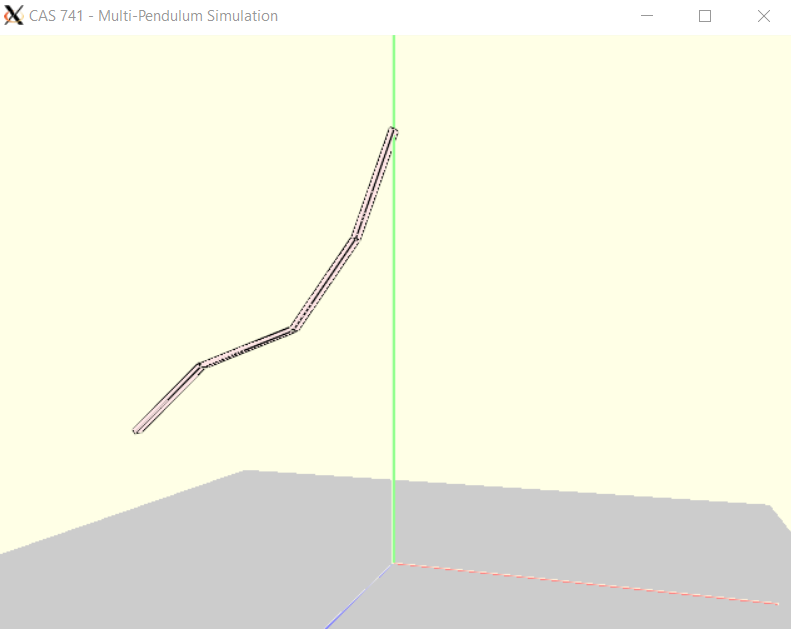
\includegraphics[width=500px]{MPSim.PNG}
	\caption{Kinetic and potential energy and simulation
	of multi-rod pendulum chain}
	\label{fig:PE-pend}
\end{figure}

\section{Simulate the plot KE and PE}

Once the command-line options loaded the simulation process. 
Please be patient, this step can take some time. 
At the end of the simulation, KE and PE will appear:

\begin{lstlisting}
$ python3 MPSim.py --nlinks 5 --gplane
Hit ESC key to quit.
Simulation reset
KE: 22.8   PE: 115.3   Total: 138.1
\end{lstlisting}
%\begin{figure}[H]
%\centering
%\includegraphics[scale=1]{Figures/(n,m)_shift.png}
%\caption{Conversion window}
%\label{fig:nm_shift}
%\end{figure}

\bibliographystyle {plainnat}
\bibliography {../../ReferenceMaterial/References}

\end{document}
